


\subsection{Funktionsstruktur und Konzeptbewertung}

Ein Konzept stellt in erster Linie einen prinzipiellen Aufbau dar und dient der Überprüfung, inwieweit die gestellten Anforderungen erfüllt werden. Da durch das Konzept die grundlegende Gestalt und die wichtigsten Merkmale festgelegt werden, ist die Konzeptphase einer der wichtigsten Abschnitte im Entwicklungsprozess. Das Gesamtkonzept lässt sich nach~\cite{Pahl_Beitz_Konstruktionslehre} folgendermaßen unterteilen:

\begin{description}
    \item[Gestaltungskonzept] Festlegung der grundlegenden Geometrie, Zuordnung der einzelnen Komponenten und Betrachtung von Stoff-, Energie- und Signalflüssen
    \item[Wirkkonzept] Beschreibung der physikalischen Effekte und deren Verknüpfung zur Erfüllung der \mbox{gestellten} Anforderungen sowie der Gestalt der Wirkflächen
    \item[Wirkfläche] Funktionale Flächen, an denen das Wirkkonzept umgesetzt wird
\end{description}

Unter Berücksichtigung der Forderungen, welche die Funktion unmittelbar beeinflussen, wurden zunächst die wesentlichen Aufgaben der Konstruktion identifiziert. Die Gesamtaufgabe ist bereits eindeutig festgelegt: Innerhalb einer von äußeren Störeinflüssen abgeschirmten Messkabine sollen Probekörper im Koppelpfad zweier Hornantennen positioniert werden. Dabei ist durch die geometrischen Abmessungen und die Verkleidung reflektiver Flächen im Inneren der Messkammer sicherzustellen, dass sich die Proben im ungestörten Fernfeld (vgl. \Kapitel\ref{cha:2}) der Antennen befinden. Festzulegen bleibt im Weiteren der genaue Aufbau der Messkabine unter Berücksichtigung der zu erreichenden Schirmung, die Gestaltung von Öffnungen und Durchführungen, die Positionierung der Antennen und Probekörper und die Auswahl geeigneter Absorber, um Hohlraumresonanzen (vgl. \Abschnitt\ref{cha:2_subsub_Hohlraumresonanzen}), Reflektionen und indirekte Kopplung (vgl. \Abschnitt\ref{cha:2_sub_Reflektion}) zu vermeiden. Mithilfe der in \Abb\ref{fig:3_Funktionsstruktur} dargestellten Funktionsstruktur wurde die Gesamtaufgabe weiter abstrahiert und gegliedert. %Die Qualifikation des Teststandes anhand des Vergleiches der durchgeführten und mit früheren Messungen ist als Teil der Auswertung nicht in der Funktionsstruktur enthalten.

\begin{figure}[ht]
    \centering
    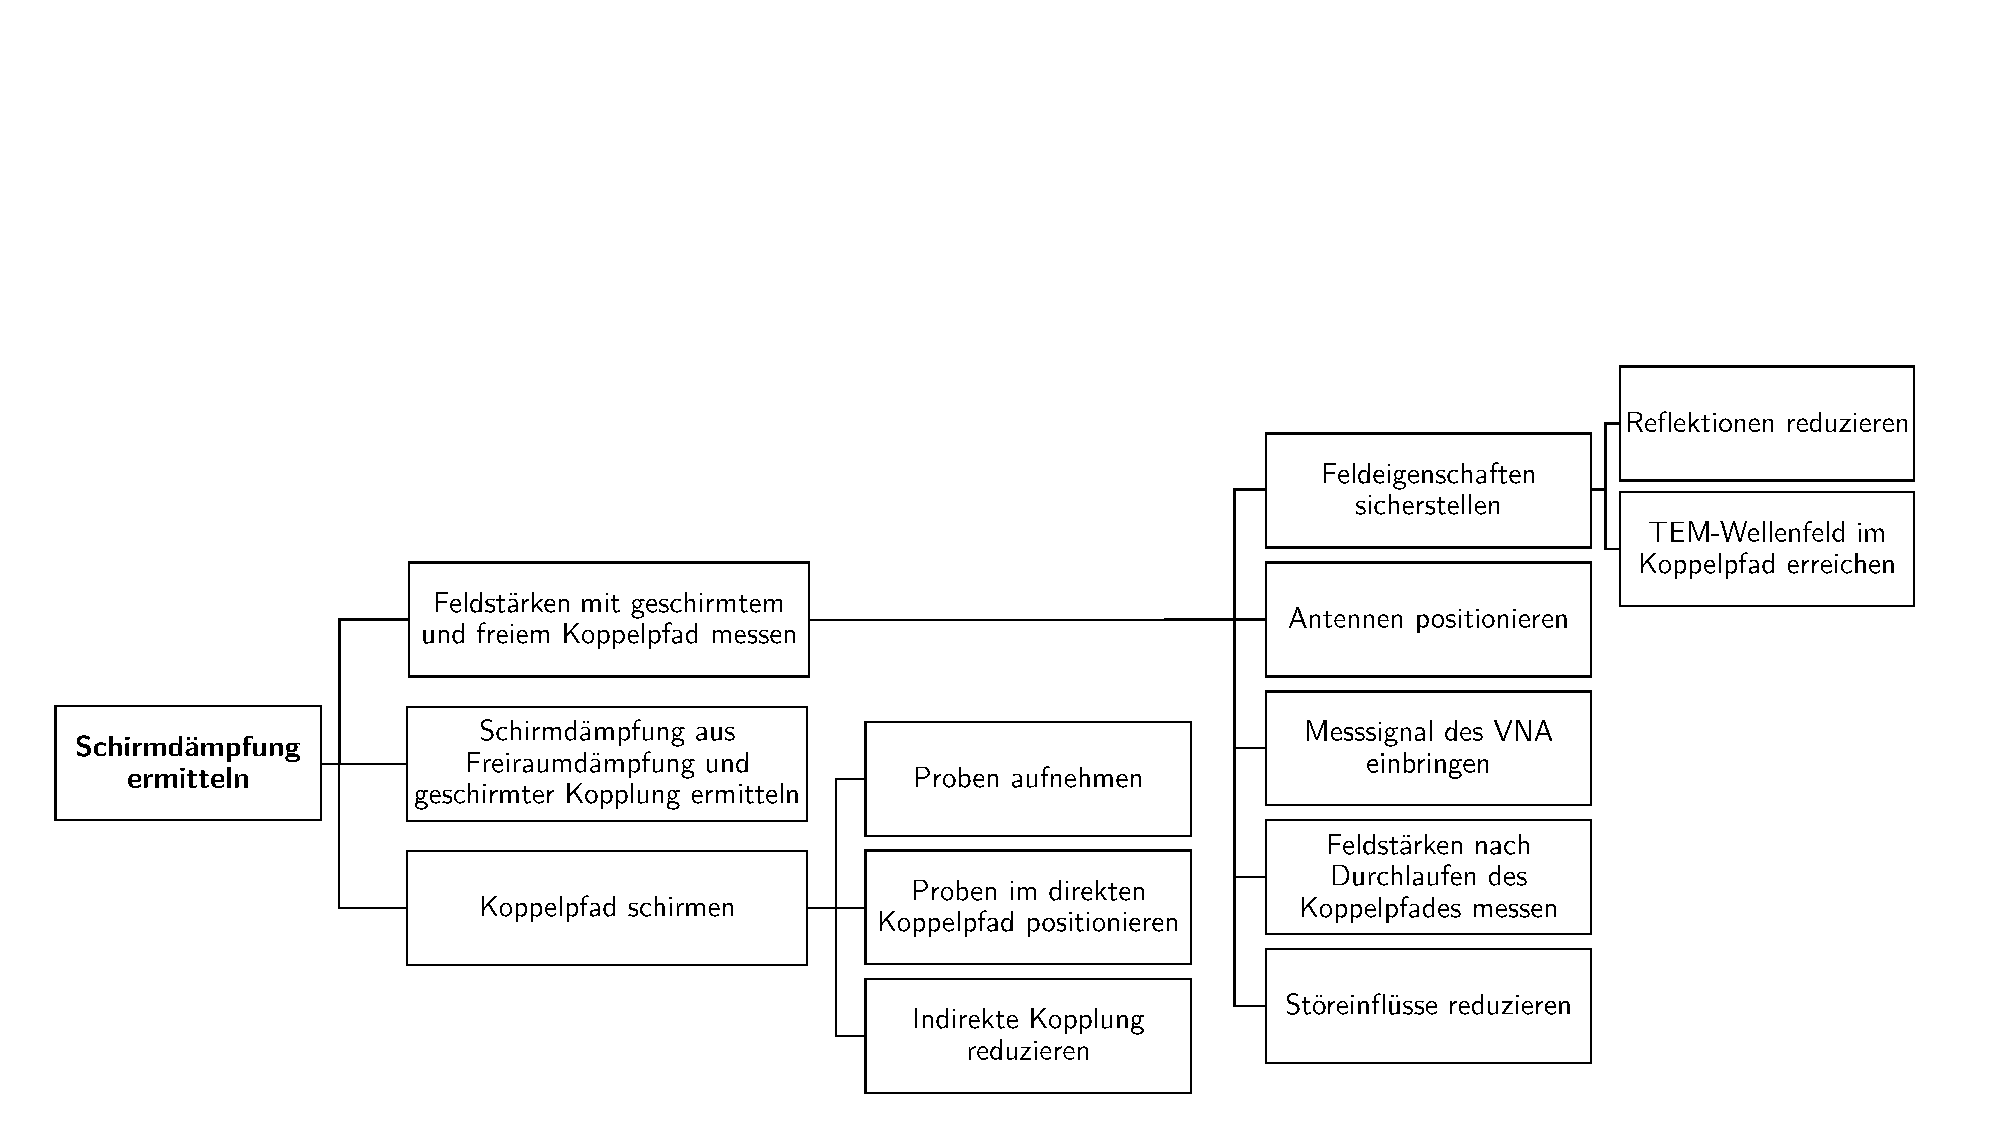
\includegraphics[page = 1, width=\textwidth, trim = 0.8cm 0.5cm 1.3cm 5.5cm, clip]{Abbildungen/Kapitel3/Funktionsstruktur.pdf}
    \caption{Funktionsstruktur der Messkabine}
    \label{fig:3_Funktionsstruktur}
\end{figure}


Auf dieser Grundlage lassen sich nun verschiedene Wirkkonzepte für die Teilstrukturen der Messkammer und deren Wirkflächen erstellen. Das Augenmerk des Designs lag dabei auf einer robusten und einfachen Geometrie der Wirkflächen bei gleichzeitiger Gewährleistung einer möglichst hohen Dichtheit gegenüber elektromagnetischer Strahlung. Letzteres kann nach der betrachteten Theorie in den \mbox{\Abschnitten}\ref{cha:2_sub_Daempfung_und_Absorption}, \ref{cha:2_sub_Reflektion} und \ref{cha:2_sub_Schirmung_ebener_Wellenfelder} durch die Herstellung eines leitfähigen Flächenkontaktes mit möglichst geringem \mbox{Kontaktwiderstand} zwischen allen Elementen der äußeren Schirmwand erreicht werden. Dies ist somit der physikalische Effekt, auf dem die Wirkkonzepte der Messkabine und der Durchführungen beruhen. 
\par
\vspace{\linespace}
Zur strukturierten und nachvollziehbaren Durchführung des Entscheidungsprozesses und der Auswahl der potenziell besten aus den vorgestellten Lösungsvarianten, kam ein Bewertungsschema zum Einsatz. Die Bewertungskriterien wurden nach dem Top-down-Vorgehen abgeleitet. Das bedeutet die Anforderungen des gesamten Versuchsstandes wurden für die einzelnen Teilsysteme detailliert~\cite{Pahl_Beitz_Konstruktionslehre}. Die gewählten Kriterien weisen die in~\cite{Pahl_Beitz_Konstruktionslehre} beschriebenen Voraussetzungen, wie unter anderem Freiheit von Dopplungen, Gegenläufigkeit und Widersprüchen sowie Gültigkeit für alle vorgestellten Varianten, auf.
\par
\vspace{\linespace}
Die Bewertung bestand aus der Anwendung eines gewichteten Punkteschemas, welches allen Kriterien Maßzahlen hinsichtlich ihrer Erfüllung durch die Konzepte zuordnete. Dies sorgte für ein vergleichsweise einfaches Bewertungsschema, welches gegenüber einer reinen Argumentenbilanz jedoch eine deutlich präzisere Entscheidung zulässt und die quantifizierbare Möglichkeit einer Wichtung bietet. Die \mbox{Bewertung} der einzelnen Konzepte erfolgte getrennt je Teilsystem des Aufbaus. Mithilfe des errechneten Gesamtwertes $G_V$ je Lösungsvariante aus den Maßzahlen $M$ und den Gewichtet $w$ konnte die Auswahl der besten Variante unmittelbar erfolgen~\cite{Pahl_Beitz_Konstruktionslehre}:

\begin{equation}
    G_{V_i} = \sum_{j=1}^{k} w_j \cdot M_{j,i}
    \label{eq:3_Gesamtwert_Variantenvergleich}
\end{equation}
\begin{equation}
    w_j \in \{\mathbb{Q} \;\vert\; 0 < w_j \leq 1\}; \qquad \sum_{j=1}^{k} w_j = 1; \qquad M_{j,i} \in \{1,\,2,\,3,\,4\}
    \label{eq:3_Wichtung_Bewertung}
\end{equation}
\begin{equation*}
    \text{\textit{k: Anzahl Kriterien; i: Variante; j: Kriterium}}
\end{equation*}

Eine höhere Maßzahl der Bewertung steht dabei stets für die jeweils bessere Variante innerhalb eines Kriteriums. Damit kann die beste Variante der jeweiligen Teilstruktur durch den höchsten Gesamtwert $G_V$ identifiziert werden. Die Wichtung erfolgte entsprechend der Kategorisierung und Wichtigkeit der jeweiligen Forderung.
\par
\vspace{\linespace}
Die Gestaltung der Probenhalterung als Teil der Messstrecke erfolgte ebenfalls im Rahmen der Konzeptphase. Die betrachteten Varianten wiesen jedoch nur geringe Unterschiede auf, sodass hier nur das gewählte Konzept als Teil des Entwurfes im \Abschnitt\ref{cha:3_Entwurf} beschrieben wird. Ähnliches gilt für die Auswahl geeigneter Absorberelemente zur Auskleidung des Innenraumes des Versuchsstandes und weitere Details, wie bspw. die Durchführungen der Antennenkabel, sodass diese und eine kurze Beschreibung der Entscheidungsgrundlage ebenfalls im \Abschnitt\ref{cha:3_Entwurf} vorgestellt werden.
%\par
%\vspace{\linespace}


\subsection{Schirmmodule des Versuchsstandes}\label{cha:3_sub_Schirmmodule_Versuchsstand}

Die Module bzw. Wände der Messkabine übernehmen die Schirmung äußerer Störeinflüsse und sind gleichzeitig Anschlussflächen zur Befestigung der Absorberelemente, Türen und Kabeldurchführungen. Bei den betrachteten Konzepten kann davon ausgegangen werden, dass ihre Schirmdämpfung im Idealfall deutlich größer als die der Durchführungen ist, sodass für die Bewertung entscheidend war, wie robust diese Schirmdämpfung gegenüber Unebenheiten und Abweichungen ist. Beispielsweise bieten mehrere Wirkflächen, die in einer Art Labyrinth im Koppelpfad angeordnet sind auch dann noch eine ausreichende Schirmung, wenn eine der Wirkflächenpaarungen nicht korrekt aufeinander liegt und damit kein leitender über der gesamten Fläche entsteht. 
\par
\vspace{\linespace}
Die \Tabelle\ref{tab_3:Konzepte_Schirmmodule} zeigt die Wirkkonzepte, für welche die Bewertung durchgeführt wurde und aus denen das finale Konzept ausgewählt wurde. 


\begin{longtable}{l p{6.55cm} p{6.55cm}}
    \caption{Wirkkonzeptskizzen der Schirmmodule des Versuchsstandes}
    \vspace{\tablespace}
    \label{tab_3:Konzepte_Schirmmodule} \\
    \toprule 
    \textbf{Bauweise}& \multicolumn{2}{l}{\textbf{Varianten}}\\
    \midrule 
    \endfirsthead 
    \caption[]{Wirkkonzeptskizzen der Schirmmodule des Versuchsstandes \emph{(Fortsetzung)}}
    \vspace{\tablespace} \\
    \toprule 
    \textbf{Bauweise}& \multicolumn{2}{l}{\textbf{Varianten}}\\
    \midrule 
    \endhead 
    \bottomrule\nopagebreak 
    \multicolumn{3}{c}{\dots}
    \endfoot 
    \bottomrule 
    \endlastfoot

         \textbf{Stahlblech} & Variante 1 & Variante 2 \\ \nopagebreak
         & \noindent\begin{minipage}{6.5cm}
                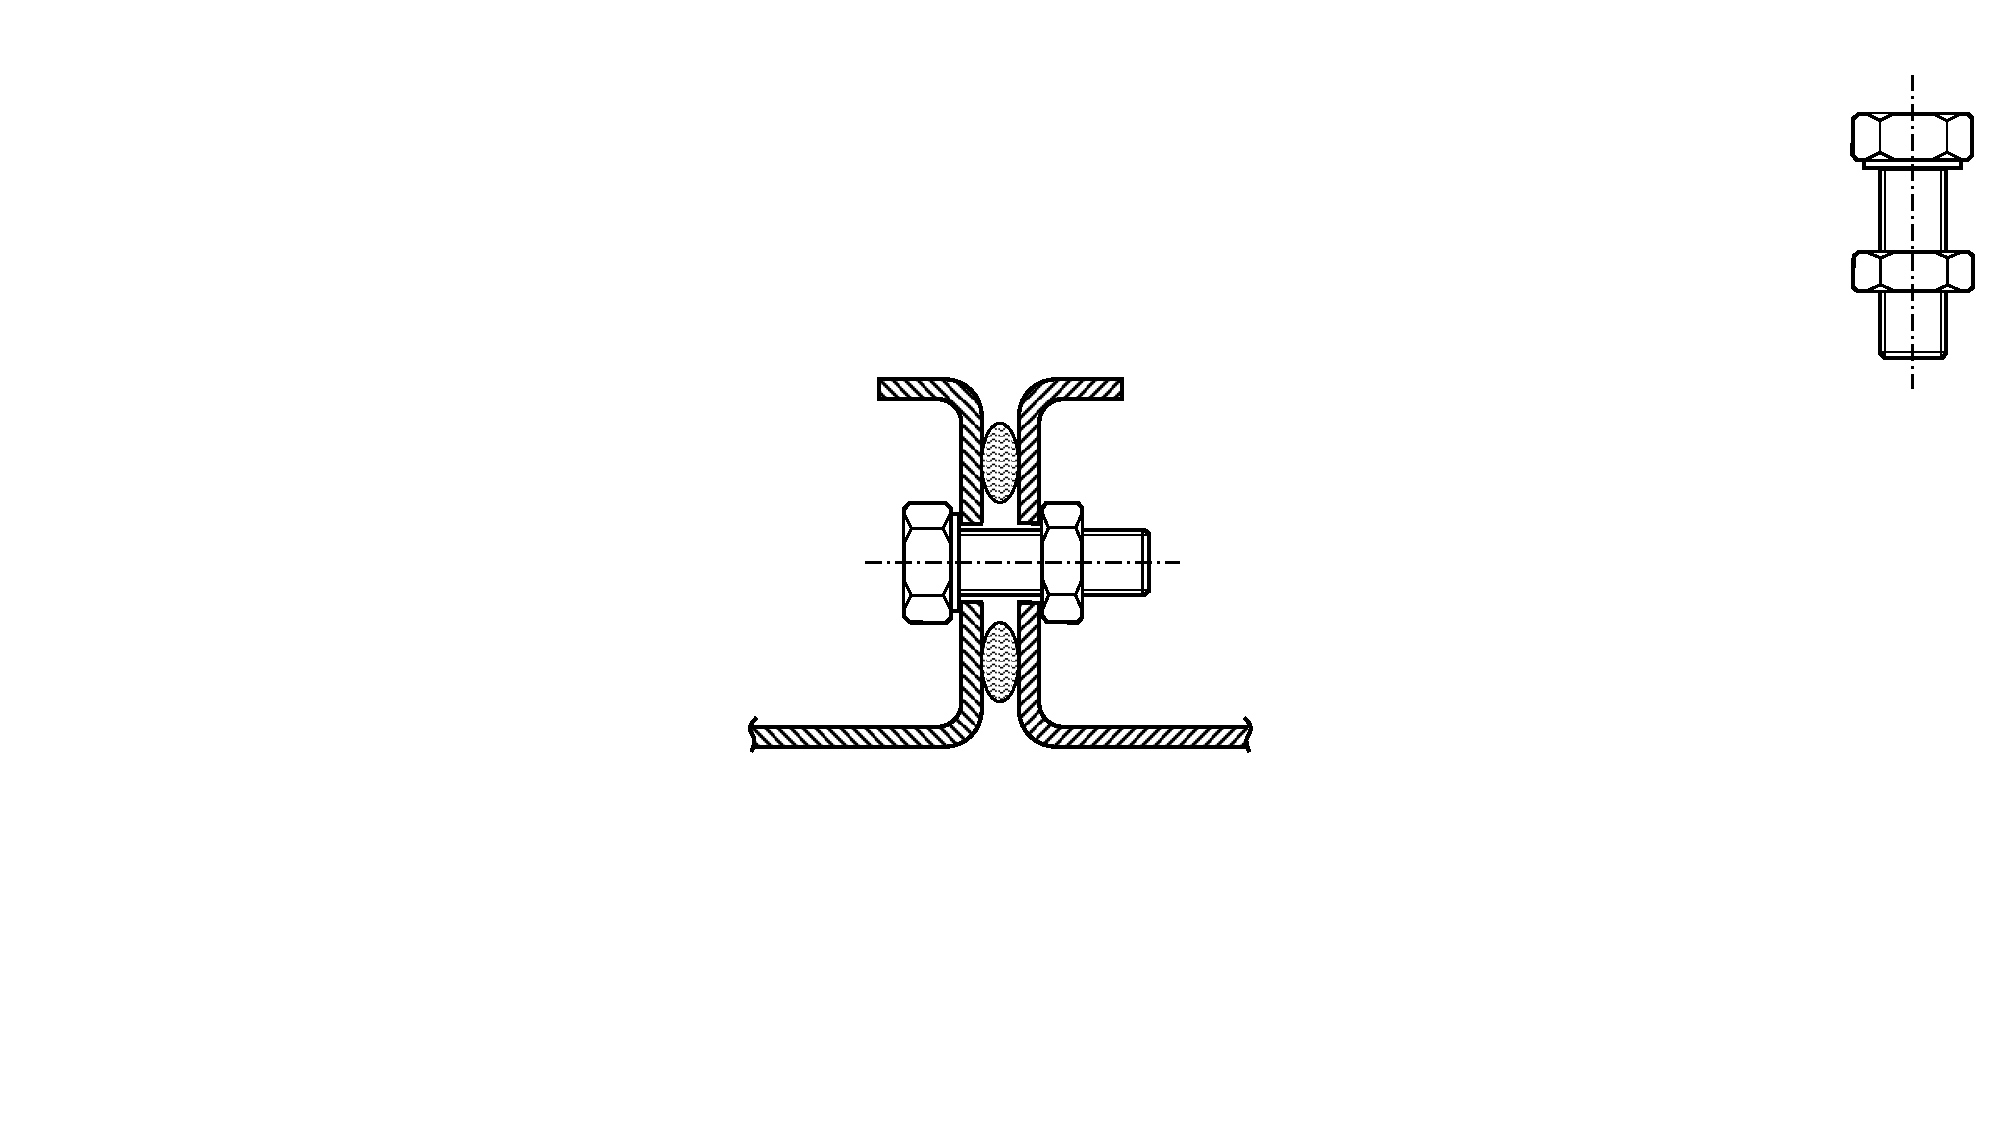
\includegraphics[page=1, width=0.95\textwidth, trim = 12cm 5.5cm 12cm 5.5cm, clip]{Abbildungen/Kapitel3/Konzepte.pdf}
        \end{minipage} &
        \noindent\begin{minipage}{6.5cm}
                \includegraphics[page=2, width=0.95\textwidth, trim = 12cm 5.5cm 12cm 5.5cm, clip]{Abbildungen/Kapitel3/Konzepte.pdf}
        \end{minipage} \\
         & Variante 3 & Variante 4 \\ \nopagebreak
         & \noindent\begin{minipage}{6.5cm}
                \includegraphics[page=3, width=0.95\textwidth, trim = 12cm 5.5cm 12cm 6.5cm, clip]{Abbildungen/Kapitel3/Konzepte.pdf}
        \end{minipage} &
        \noindent\begin{minipage}{6.5cm}
                \includegraphics[page=4, width=0.95\textwidth, trim = 12cm 6cm 12cm 5.5cm, clip]{Abbildungen/Kapitel3/Konzepte.pdf}
        \end{minipage} \\
    \midrule
         \textbf{Sandwich} & Variante 5 & Variante 6 \\ \nopagebreak 
         & \noindent\begin{minipage}{6.5cm}
                \includegraphics[page=5, width=0.95\textwidth, trim = 12.5cm 6cm 12cm 6cm, clip]{Abbildungen/Kapitel3/Konzepte.pdf}
        \end{minipage} &
        \noindent\begin{minipage}{6.5cm}
                \includegraphics[page=6, width=0.95\textwidth, trim = 14cm 7cm 10cm 7cm, clip]{Abbildungen/Kapitel3/Konzepte.pdf}
        \end{minipage} \\
         & Variante 7 & Variante 8  \\ \nopagebreak
         & \noindent\begin{minipage}{6.5cm}
                \includegraphics[page=7, width=0.95\textwidth, trim = 13cm 7cm 12cm 7cm, clip]{Abbildungen/Kapitel3/Konzepte.pdf}
        \end{minipage} &
        \noindent\begin{minipage}{6.5cm}
                \includegraphics[page=8, width=0.95\textwidth, trim = 8.5cm 3cm 12cm 5.5cm, clip]{Abbildungen/Kapitel3/Konzepte.pdf}
        \end{minipage} \\
\end{longtable}


\par
\vspace{\linespace}
Die Bewertung der verschiedenen Wirkkonzepte erfolgte anhand der nachstehenden \acp{K}: 

\begin{tabular}{l l}
    \centering
    \hspace*{1cm} \parbox[c][3cm]{7cm}{
        \begin{itemize}[]
            \item \textbf{K\textsubscript{1}} Materialkosten
            \item \textbf{K\textsubscript{2}} Fertigungsaufwand
            \item \textbf{K\textsubscript{3}} Robustheit gegenüber Lecks
        \end{itemize}
    }&
    \parbox[c]{7cm}{
        \begin{itemize}[]
            \item \textbf{K\textsubscript{4}} Montageaufwand
            \item \textbf{K\textsubscript{5}} Stabilität
            \item \textbf{K\textsubscript{6}} Materialverfügbarkeit
        \end{itemize}
    }
\end{tabular}

In der \Tabelle\ref{tab:3_Module_Messkabine} ist die Konzeptbewertung der Modulwände und die Auswertung nach den \mbox{\Gleichungen} \eqref{eq:3_Gesamtwert_Variantenvergleich} und \eqref{eq:3_Wichtung_Bewertung} dargestellt.


\begin{table}[ht]
    \centering
    \renewcommand{\arraystretch}{1.3}
    \caption{Konzeptbewertung der Schirmmodule des Versuchsstandes}
    \vspace{\tablespace}
    \label{tab:3_Module_Messkabine}
    \begin{tabularx}{\textwidth}{p{3cm} r C{1cm} C{1cm} C{1cm} C{1cm} C{1cm} C{1cm} C{1.5cm}}
        \toprule
        \multirow{2}{*}{\textbf{Variante i}} & \textbf{Kriterien K\textsubscript{j}} & \textbf{K\textsubscript{1}} & \textbf{K\textsubscript{2}} & \textbf{K\textsubscript{3}} & \textbf{K\textsubscript{4}} & \textbf{K\textsubscript{5}} & \textbf{K\textsubscript{6}} & \textbf{Summe} \\
         & Gewichte w\textsubscript{j} & 0,1 & 0,1 & 0,25 & 0,1 & 0,2 & 0,25 & \textbf{G\textsubscript{V}} \\
         \midrule
         \multicolumn{2}{l}{Variante 1} & 1 & 2 & 2 & 2 & 3 & 3 & 2,35 \\
         \multicolumn{2}{l}{Variante 2} & 2 & 3 & 2 & 3 & 2 & 3 & 2,45 \\
         \multicolumn{2}{l}{Variante 3} & 1 & 1 & 4 & 3 & 3 & 2 & 2,6 \\
         \multicolumn{2}{l}{Variante 4} & 2 & 2 & 4 & 4 & 2 & 2 & 2.7 \\
         \multicolumn{2}{l}{Variante 5} & 2 & 4 & 3 & 1 & 2 & 2 & 2,35 \\
         \multicolumn{2}{l}{Variante 6} & 4 & 4 & 4 & 2 & 3 & 1 & 2,85 \\
         \multicolumn{2}{l}{Variante 7} & 3 & 4 & 3 & 2 & 4 & 4 & 3,45 \\
         \multicolumn{2}{l}{Variante 8} & 3 & 2 & 1 & 3 & 1 & 4 & 2,25 \\
         \bottomrule
    \end{tabularx}
\end{table}

Mit L-Profilen verschraubte Sandwichpaneele stellen somit für den Aufbau einer Absorberkammer im Rahmen dieser Arbeit die beste Lösung dar. Die mehrlagige Struktur gewährleistet aufgrund zusätzlicher Reflektion zwischen den Deckblechen eine deutlich größere Schirmung bei gleichem Materialaufwand im Vergleich zu einfachen Blechen. Weiterhin kann auch am realen Schirm von einem niedrigeren Felddurchgriff ausgegangen werden, da sich stets zwei Wirkflächen im Koppelpfad befinden. Die Wabenstruktur im Inneren sorgt außerdem für eine sehr hohe Biegefestigkeit im Verhältnis zur Masse~\cite{Alucore-Datenblatt}. Aus diesen Gründen wird der Grundaufbau mithilfe von Sandwichpaneelen entsprechend der Variante~7 realisiert.

%Sandwichpaneele oder Wabenkernplatten mit Deckblechen <-- Wahl
%Mehrfachschirmung --> gleiche Schirmung bei geringerem Materialaufwand durch zusätzliche Reflektion innerhalb der Struktur (EMV-gerechtes Gerätedesign) + besseres Herabsetzen des Felddurchgriffes beim realen Schirm an Öffnungen, etc.  




\subsection{Durchführungen}\label{cha:3_sub_Durchfuehrungen}

Die Türen des Versuchsstandes erlauben im Betrieb vor allem den Zugriff auf die Antennen und den Wechsel der Probekörper. Wie jede Öffnung in einer Schirmwand stellen sie neben den Kabeldurchführungen und den Anschlussstellen der Kammerwände eine der kritischsten Stellen in Bezug auf die erreichbare Schirmung der Messkabine dar (vgl. \Abschnitt\ref{cha:2_sub_Schirmung_ebener_Wellenfelder}). Aus diesem Grund wurden im Entwurf solche Konzepte, die eine Schirmung nur aufgrund einer Labyrinthwirkung ohne leitenden Flächenkontakt erreichen, nicht in Betracht gezogen. Diese weisen im Vergleich zu den nachfolgend vorgestellten Konzepten eine deutlich geringere Schirmdämpfung auf~\cite{Design_of_shielded_enclosures}.
\par
\vspace{\linespace}
In Anlehnung an die Gestaltungsbeispiele in~\cite{EM_Schirmung, Design_of_shielded_enclosures} wurden die in \Tabelle\ref{tab_3:Konzepte_Durchfuehrungen} gezeigten Konzepte ausgearbeitet. Bei der Art der hauptsächlich verwendeten Dichtungen kann grundsätzlich zwischen Kontaktfederstreifen aus Kupfer-Beryllium-Legierungen und metallischen Gestrickdichtungen mit oder ohne Elastomer-Kern unterschieden werden~\cite{EM_Schirmung}, welche grundsätzlich über unterschiedliche Eigenschaften verfügen. Deshalb wurden für die Konzeptbewertung beide Varianten in unterschiedlichen Konfigurationen herangezogen.



\begin{longtable}{l p{6.55cm} p{6.55cm}}
    \caption{Wirkkonzeptskizzen der Durchführungen des Versuchsstandes}
    \vspace{\tablespace}
    \label{tab_3:Konzepte_Durchfuehrungen} \\
    \toprule 
    \textbf{Bauweise}& \multicolumn{2}{l}{\textbf{Varianten}}\\
    \midrule 
    \endfirsthead 
    \caption[]{Wirkkonzeptskizzen der Durchführungen des Versuchsstandes \emph{(Fortsetzung)}}
    \vspace{\tablespace} \\
    \toprule 
    \textbf{Bauweise}& \multicolumn{2}{l}{\textbf{Varianten}}\\
    \midrule 
    \endhead 
    \bottomrule\nopagebreak 
    \multicolumn{3}{c}{\dots}
    \endfoot 
    \bottomrule 
    \endlastfoot

         \begin{minipage}{2cm}\vspace*{5pt}\textbf{Kontakt-federstreifen}\end{minipage} & Variante 1 & Variante 2 \\ \nopagebreak
          & \noindent\begin{minipage}{6.5cm}
                \includegraphics[page=9, width=0.95\textwidth, trim = 12.5cm 7.5cm 9.5cm 6.5cm, clip]{Abbildungen/Kapitel3/Konzepte.pdf}
        \end{minipage} &
        \noindent\begin{minipage}{6.5cm}
                \includegraphics[page=10, width=0.95\textwidth, trim = 12.5cm 9cm 12cm 5cm, clip]{Abbildungen/Kapitel3/Konzepte.pdf}
        \end{minipage} \\
        & & \\
    \midrule
         \begin{minipage}{2cm}\vspace*{5pt}\textbf{Gestrick-dichtungen}\end{minipage} & Variante 3 & Variante 4 \\ \nopagebreak 
         & \noindent\begin{minipage}{6.5cm}
                \includegraphics[page=11, width=0.95\textwidth, trim = 12.5cm 7.5cm 9.5cm 6.5cm, clip]{Abbildungen/Kapitel3/Konzepte.pdf}
        \end{minipage} &
        \noindent\begin{minipage}{6.5cm}
                \includegraphics[page=12, width=0.95\textwidth, trim = 12.5cm 6.5cm 11.5cm 7cm, clip]{Abbildungen/Kapitel3/Konzepte.pdf}
        \end{minipage} \\
         & Variante 5 & Variante 6  \\ \nopagebreak
         & \noindent\begin{minipage}{6.5cm}
                \includegraphics[page=13, width=0.95\textwidth, trim = 10.5cm 8cm 12.5cm 5cm, clip]{Abbildungen/Kapitel3/Konzepte.pdf}
        \end{minipage} &
        \noindent\begin{minipage}{6.5cm}
               \includegraphics[page=14, width=0.95\textwidth, trim = 10.5cm 8cm 13cm 5cm, clip]{Abbildungen/Kapitel3/Konzepte.pdf}
        \end{minipage} \\
\end{longtable}

Die Bewertung wurde mithilfe der Richtlinien in~\cite{EM_Schirmung, Design_of_shielded_enclosures} durchgeführt und erfolgte anhand der nachstehenden Kriterien:


\begin{tabular}{l l}
    \hspace*{0.5cm}\parbox[c]{6.5cm}{
        \begin{itemize}[]
            \item \textbf{K\textsubscript{1}} Materialkosten
            \item \textbf{K\textsubscript{2}} Erreichbare Schirmdämpfung
            \item \textbf{K\textsubscript{3}} Beständigkeit der Elastizität
            \item[]
        \end{itemize}
    }&
    \parbox[c]{8cm}{
        \begin{itemize}[]
            \item \textbf{K\textsubscript{4}} Anfälligkeit gegen mechanische Beschädigung
            \item \textbf{K\textsubscript{5}} Robustheit gegenüber Spaltmaßtoleranzen
            \item \textbf{K\textsubscript{6}} Durchdringung von Oxidschichten und Selbstreinigung der Oberflächen
        \end{itemize}
    }
\end{tabular}

Entscheidend für die Spaltmaßtoleranz ist beispielsweise, dass der Zusammenhang der Dichtungshöhe und der notwendigen Anpresskraft bei Vollmetallgestrickdichtungen stark nichtlinear ist~\cite{EM_Schirmung}. \mbox{Geringe} Überschreitungen führen hier gegebenenfalls schon zur Unterbrechung des elektrischen Kontaktes. Gestrickdichtungen mit Elastomer-Kern gleichen diesen Nachteil teilweise aus, besitzen jedoch insgesamt eine geringere Federkonstante als Vollmetallgestricke und Kontaktfedern. Dadurch durchdringen sie Oberflächenschichten kaum, was bei den verwendeten Aluminiumwänden entscheidend für den elektrischen Kontakt ist. Weiterhin verlieren sie bei dauerhaftem Anpressen schnell ihre Elastizität. In der \Tabelle\ref{tab:3_Durchfuehrungen} ist das Ergebnis der Konzeptbewertung der Durchführungen ersichtlich.
\par
\vspace{\linespace}

\begin{table}[ht]
    \centering
    \renewcommand{\arraystretch}{1.3}
    \caption{Konzeptbewertung der Durchführungen des Versuchsstandes}
    \vspace{\tablespace}
    \label{tab:3_Durchfuehrungen}
    \begin{tabularx}{\textwidth}{p{3cm} r C{1cm} C{1cm} C{1cm} C{1cm} C{1cm} C{1cm} C{1.5cm}}
        \toprule
        \multirow{2}{*}{\textbf{Variante i}} & \textbf{Kriterien K\textsubscript{j}} & \textbf{K\textsubscript{1}} & \textbf{K\textsubscript{2}} & \textbf{K\textsubscript{3}} & \textbf{K\textsubscript{4}} & \textbf{K\textsubscript{5}} & \textbf{K\textsubscript{6}} & \textbf{Summe} \\
        & Gewichte w\textsubscript{j} & 0,1 & 0,25 & 0,1 & 0,1 & 0,25 & 0,2 & \textbf{G\textsubscript{V}} \\
         \midrule
         \multicolumn{2}{l}{Variante 1} & 2 & 3 & 4 & 2 & 4 & 4 & 3,35 \\
         \multicolumn{2}{l}{Variante 2} & 1 & 4 & 4 & 1 & 3 & 4 & 3,15 \\
         \multicolumn{2}{l}{Variante 3} & 4 & 1 & 3 & 4 & 1 & 1 & 1,8 \\
         \multicolumn{2}{l}{Variante 4} & 1 & 3 & 1 & 3 & 3 & 3 & 2.6 \\
         \multicolumn{2}{l}{Variante 5} & 3 & 2 & 3 & 4 & 2 & 2 & 2,4 \\
         \multicolumn{2}{l}{Variante 6} & 2 & 2 & 3 & 4 & 1 & 1 & 1,85 \\
         \bottomrule
    \end{tabularx}
    \vspace{\tablespace}
\end{table}

Kontaktfederstreifen eignen sich für die vorliegende Anwendung vor allem aufgrund ihrer Robustheit gegenüber Spaltmaßtoleranzen und der guten Selbstreinigung der Wirkflächen. Die Herstellung eines niederohmigen Kontaktes erfordert die Entfernung oberflächlicher Aluminiumoxidschichten auf den Modulwänden durch hohe Kontaktkräfte oder, im Falle der Kontaktstreifen, eine Relativbewegung der Oberflächen bei jedem Schließvorgang. Messerkontakttüren bieten zwar die höchste erreichbare Schirmdämpfung, sind andererseits aber anfälliger für mechanische Beschädigung und benötigen eine deutlich aufwendigere Verschlussmechanik. Deshalb wird der Verschluss nach Variante~1 umgesetzt.

%Kontaktfederstreifen beste Variante
%Geringe Beständigkeit vor allem Nachteil --> kontrollieren, vorsichtig umgehen und ggf. in regelmäßigen Abständen austauschen
%Messerkontakt deutlich aufwendiger und anfälliger gegen geringe Abweichungen aufgrund der komplizierteren Verschlussmechanik/Bewegungskurve der Tür, damit auch ordentlich schließt (ggf. in EMV nach Formulierung schauen)